\chapter[Harald is King]{
    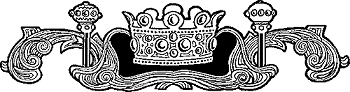
\includegraphics[width=9.3cm]{viking-tales/022}\\
    Harald is King}

\lettrine{N}{ow} when Harald was ten years old his father, King Halfdan,
died. An old book that tells about Harald says that then ``he was the
biggest of all men, the strongest, and the fairest to look upon.'' That
about a boy ten years old! But boys grew fast in those days for they were
out of doors all the time, running, swimming, leaping on skees, and
hunting in the forest. All that makes big, manly boys.

So now King Halfdan was dead and buried, and Harald was to be king. But
first he must drink his father's funeral ale.

``Take down the gay tapestries that hang in the feast hall,'' he said to
the thralls. ``Put up black and gray ones. Strew the floor with pine
branches. Brew twenty tubs of fresh ale and mead. Scour every dish until
it shines.''

Then Harald sent messengers all over that country to his kinsmen and
friends.

``Bid them come in three months' time to drink my father's funeral
ale,'' he said. ``Tell them that no one shall go away empty-handed.''

So in three months men came riding up at every hour. Some came in boats.
But many had ridden far through mountains, swimming rivers; for there
were few roads or bridges in Norway. On account of that hard ride no
women came to the feast.

At nine o'clock in the night the feast began. The men came walking in at
the west end of the hall.\footnote{See note about feast hall on
page~\pageref{feast-hall}.} The great bonfires down the middle of the
room were flashing light on everything. The clean smell of this
wood-smoke and of the pine branches on the floor was pleasant to the
guests. Down each side of the hall stretched long, backless benches, with
room for three hundred men. In the middle of each side rose the high
seat, a great carved chair on a platform. All along behind the benches
were the black and gray draperies. Here hung the shields of the guests;
for every man, when he was given his place, turned and hung his shield
behind him and set his tall spear by it. So on each wall there was a long
row of gay shields, red and green and yellow, and all shining with gold
or bronze trimmings. And higher up there was another row of gleaming
spear-points. Above the hall the rafters were carved and gaily painted,
so that dragons seemed to be crawling across, or eagles seemed to be
swooping down.

The guests walked in laughing and talking with their big voices so that
the rafters rang. They made the hall look all the brighter with their
clothes of scarlet and blue and green, with their flashing golden
bracelets and head-bands and sword-scabbards, with their flying hair of
red or yellow.

Across the east end of the hall was a bench. When the men were all in,
the queen, Harald's mother, and the women who lived with her, walked in
through the east door and sat upon this bench.

Then thralls came running in and set up the long tables\footnote{See note
about tables on page~\pageref{tables}.} before the benches. Other thralls
ran in with large steaming kettles of meat. They put big pieces of this
meat into platters of wood and set it before the men. They had a few
dishes of silver. These they put before the guests at the middle of the
tables; for the great people sat here near the high seats.

When the meat came, the talking stopped; for Norsemen ate only twice a
day, and these men had had long rides and were hungry. Three or four
persons ate from one platter and drank from the same big bowl of milk.
They had no forks, so they ate from their fingers and threw the bones
under the table among the pine branches. Sometimes they took knives from
their belts to cut the meat.

When the guests sat back satisfied, Harald called to the thralls:

``Carry out the tables.''

So they did and brought in two great tubs of mead and set one at each
end of the hall. Then the queen stood up and called some of her women.
They went to the mead tubs. They took the horns, when the thralls had
filled them, and carried them to the men with some merry word. Perhaps
one woman said as she handed a man his horn:

``This horn has no feet to be set down upon. You must drink it at one
draught.''

Perhaps another said:

``Mead loves a merry face.''

The women were beautiful, moving about the hall. The queen wore a
trailing dress of blue velvet with long flowing sleeves. She had a short
apron of striped Arabian silk with gold fringe along the bottom. From
her shoulders hung a long train of scarlet wool embroidered in gold.
White linen covered her head. Her long yellow hair was pulled around at
the sides and over her breast and was fastened under the belt of her
apron. As she walked, her train made a pleasant rustle among the pine
branches. She was tall and straight and strong. Some of her younger
women wore no linen on their heads and had their white arms bare, with
bracelets shining on them. They, too, were tall and strong.

All the time men were calling across the fire to one another asking news
or telling jokes and laughing.

An old man, Harald's uncle, sat in the high seat on the north side. That
was the place of honor. But the high seat on the south side was empty;
for that was the king's seat. Harald sat on the steps before it.

The feast went merrily until long after midnight. Then the thralls took
some of the guests to the guest house to sleep, and some to the beds
around the sides of the feast hall. But some men lay down on the benches
and drew their cloaks over themselves.

On the next night there was another feast. Still Harald sat on the step
before the high seat. But when the tables were gone and the horns were
going around, he stood up and raised high a horn of ale and said loudly:

``This horn of memory I drink in honor of my father, Halfdan, son of
Gudrod, who sits now in Valhalla. And I vow that I will grind my
father's foes under my heel.''

Then he drank the ale and sat down in the king's high seat, while all
the men stood up and raised their horns and shouted:

``King Harald!''

And some cried:

``That was a brave vow.''

\begin{figure}
    \centering
    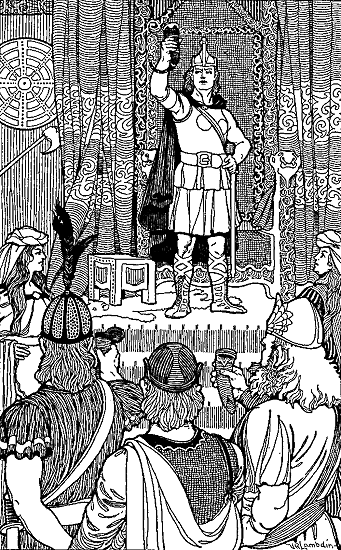
\includegraphics[width=9.1cm]{viking-tales/023}
    \caption{``I vow that I will grind my father's foes under my heel''}
\end{figure}

And Harald's uncle called out:

``A health to King Harald!''

And they all drank it.

Then a man stood up and said:

``Hear my song of King Halfdan!'' for this man was a skald.

``Yes, the song!'' shouted the men, and Harald nodded his head.

So the skald took down his great harp from the wall behind him and went
and stood before Harald. The bottom of the harp rested on the floor, but
the top reached as high as the skald's shoulders. The brass frame shone
in the light. The strings were some of gold and some of silver. The man
struck them with his hand and sang of King Halfdan, of his battles, of
his strong arm and good sword, of his death, and of how men loved him.

When he had finished, King Harald took a bracelet from his arm and gave
it to him, saying:

``Take this as thanks for your good song.''

The guests stayed the next day and at night there was another feast.
When the mead horns were going around, King Harald stood up and spoke:

``I said that no man should go away empty-handed from drinking my
father's funeral ale.''

He beckoned the thralls, and they brought in a great treasure-chest and
set it down by the high seat. King Harald opened it and took out rich
gifts--capes and sword-belts and beautiful cloth and bracelets and gold
cloak-pins. These he sent about the hall and gave something to every
man. The guests wondered at the richness of his gifts.

``This young king has an open hand,'' they said, ``and deep
treasure-chests.''

After breakfast the next morning the guests went out and stood by their
horses ready to go, but before they mounted, thralls brought a horn of
mead to each man. That was called the stirrup-horn, because after they
drank it the men put their feet to the stirrups and sprang upon their
horses and started. King Harald and his people rode a little way with
them.

All men said that that was the richest funeral feast that ever was held.
